\chapter{Supporting Information for the Ewald Embedded Cluster}

\label{app:ew}
\section{Crystal Structures}
\label{app:sec:cryst_struct}

The experimental crystal structures for HC1 and HC2 are accessible on the Cambridge Structural Database with codes 941991 and 1061608 respectively.\cite{Zhang2015}

\section{Absorption and Emission Spectra}
\label{app:sec:spectra}

To consider the effect of vibrations on the position of the absorption and emission maxima, we simulate both spectra with the nuclear ensemble approach as implemented in \texttt{Newton-X}.\cite{Crespo-Otero2012,newtonx} They are shown in Figure \ref{fig:spec}. For each scheme, the monomer was first optimised to the \textbf{FC} and \textbf{K*} geometries for absorption and emission. The vibrational modes were calculated using $\omega$B97X-D/6-311++G(d,p) in \texttt{Gaussian}\cite{g16} in the presence of the point charges from the embedding model. 

\begin{figure}[H]
%\centering
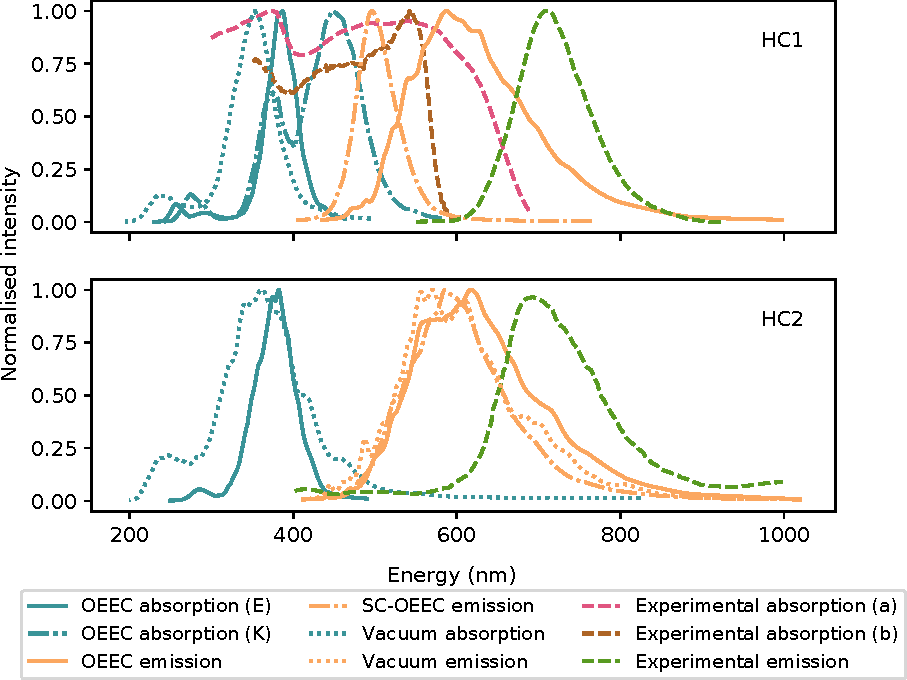
\includegraphics[width=\textwidth]{Appendices/A/spectra.pdf}
\caption{Absorption and emission spectra for both molecules with experimental data\cite{Zhang2015} for comparison. The experimental emission for HC2 is smoothed with a Savitzky-Golay filter.}
\label{fig:spec}
\end{figure}


\section{Population Analysis for Aggregates}
\label{app:sec:pop_analysis_aggregates}

RESP charges respond directly to the electrostatic environment of the atom. As such they are a measure of the quality of the embedding method. In Figure \ref{fig:chargesFC} we compare the RESP charges of notable atoms on monomers embedded in different charge backgrounds to those calculated in tetramers embedded using \EEC{}. In this case the central molecule is in the \textbf{FC} geometry. The results for \textbf{K*} are in Figure \ref{fig:chargesK}.


\begin{figure}[H]
%\centering
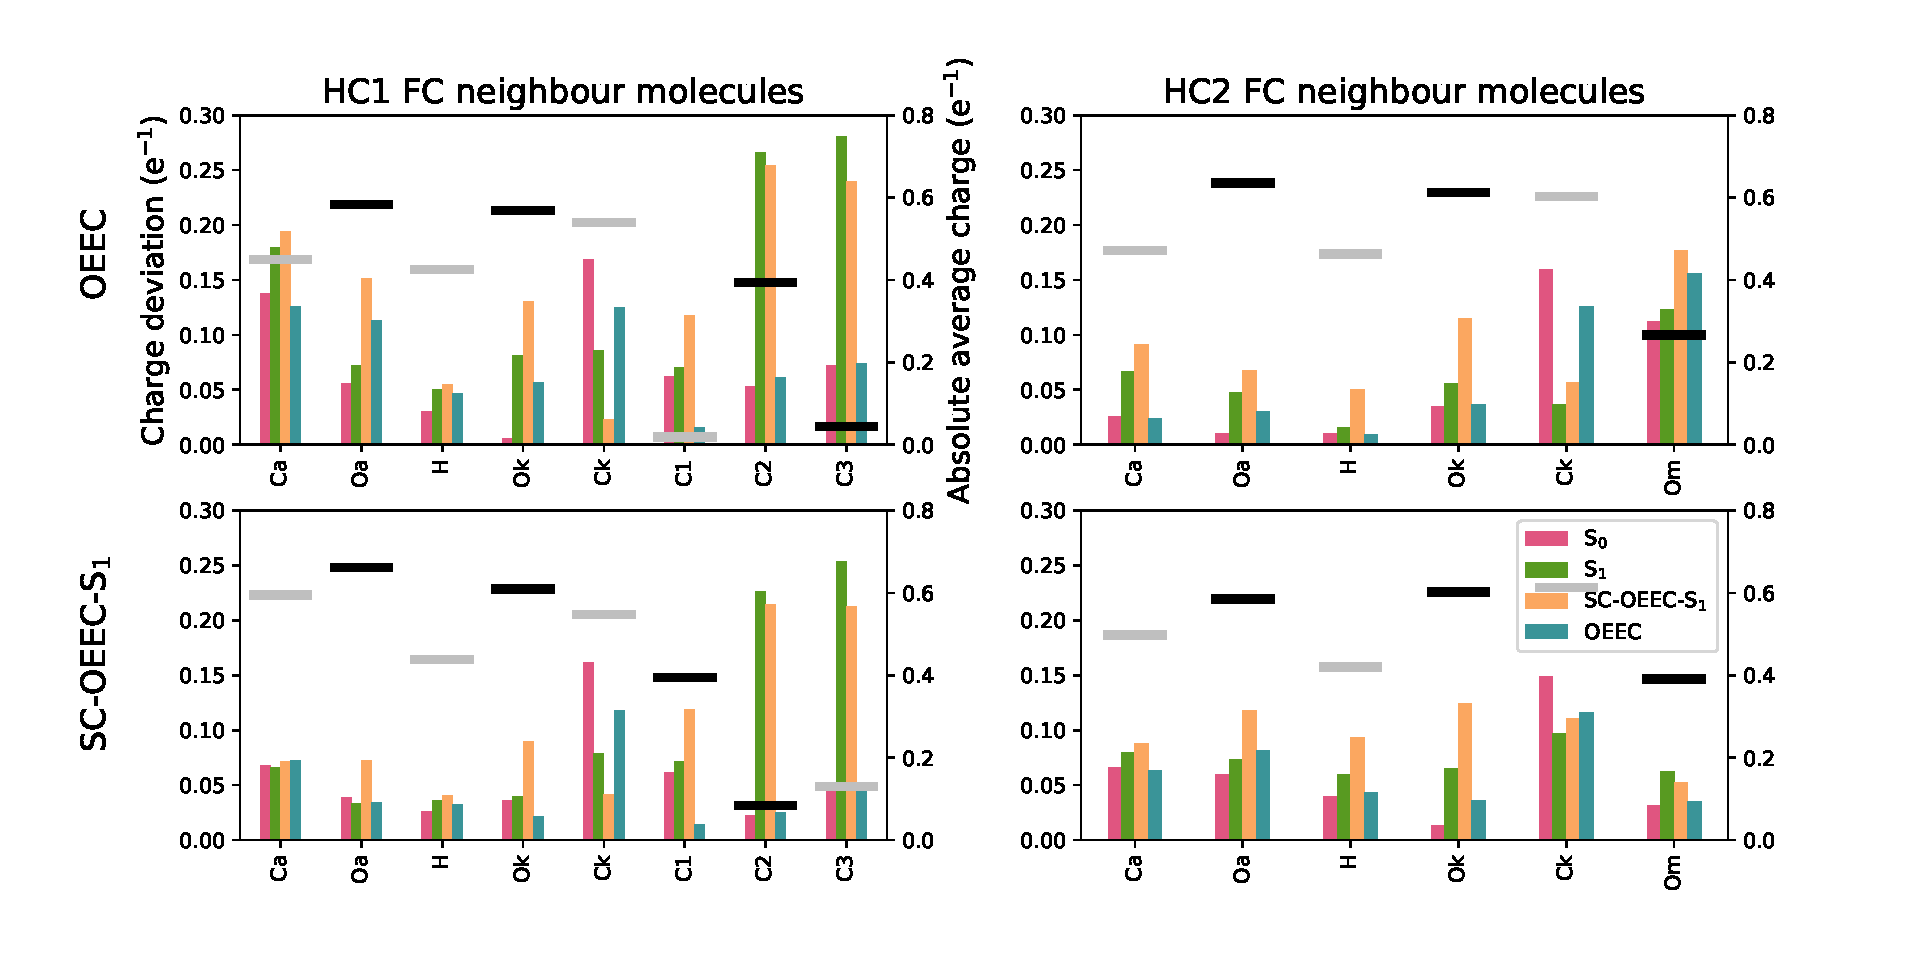
\includegraphics[width=\textwidth]{Appendices/A/just_FC.pdf}
\caption{Deviation of charge on notable atoms from the explicitly calculated tetramer with the relaxing molecule in \textbf{FC} geometry. In the top row, the molecule is optimised with \EEC{} and in the bottom with \SCEEC{}-S$_1$. We compare the charge obtained from the monomer population analysis of in vacuum S$_0$, S$_1$ and in EEC and \SCEEC{}-S$_1$. The absolute average charge in the tetramer is indicated by horizontal ticks, positive values are in grey and negative ones in black. The atom labels are the ones found in Figure 1 of the main text.}
\label{fig:chargesFC}
\end{figure}


\begin{figure}[H]
%\centering
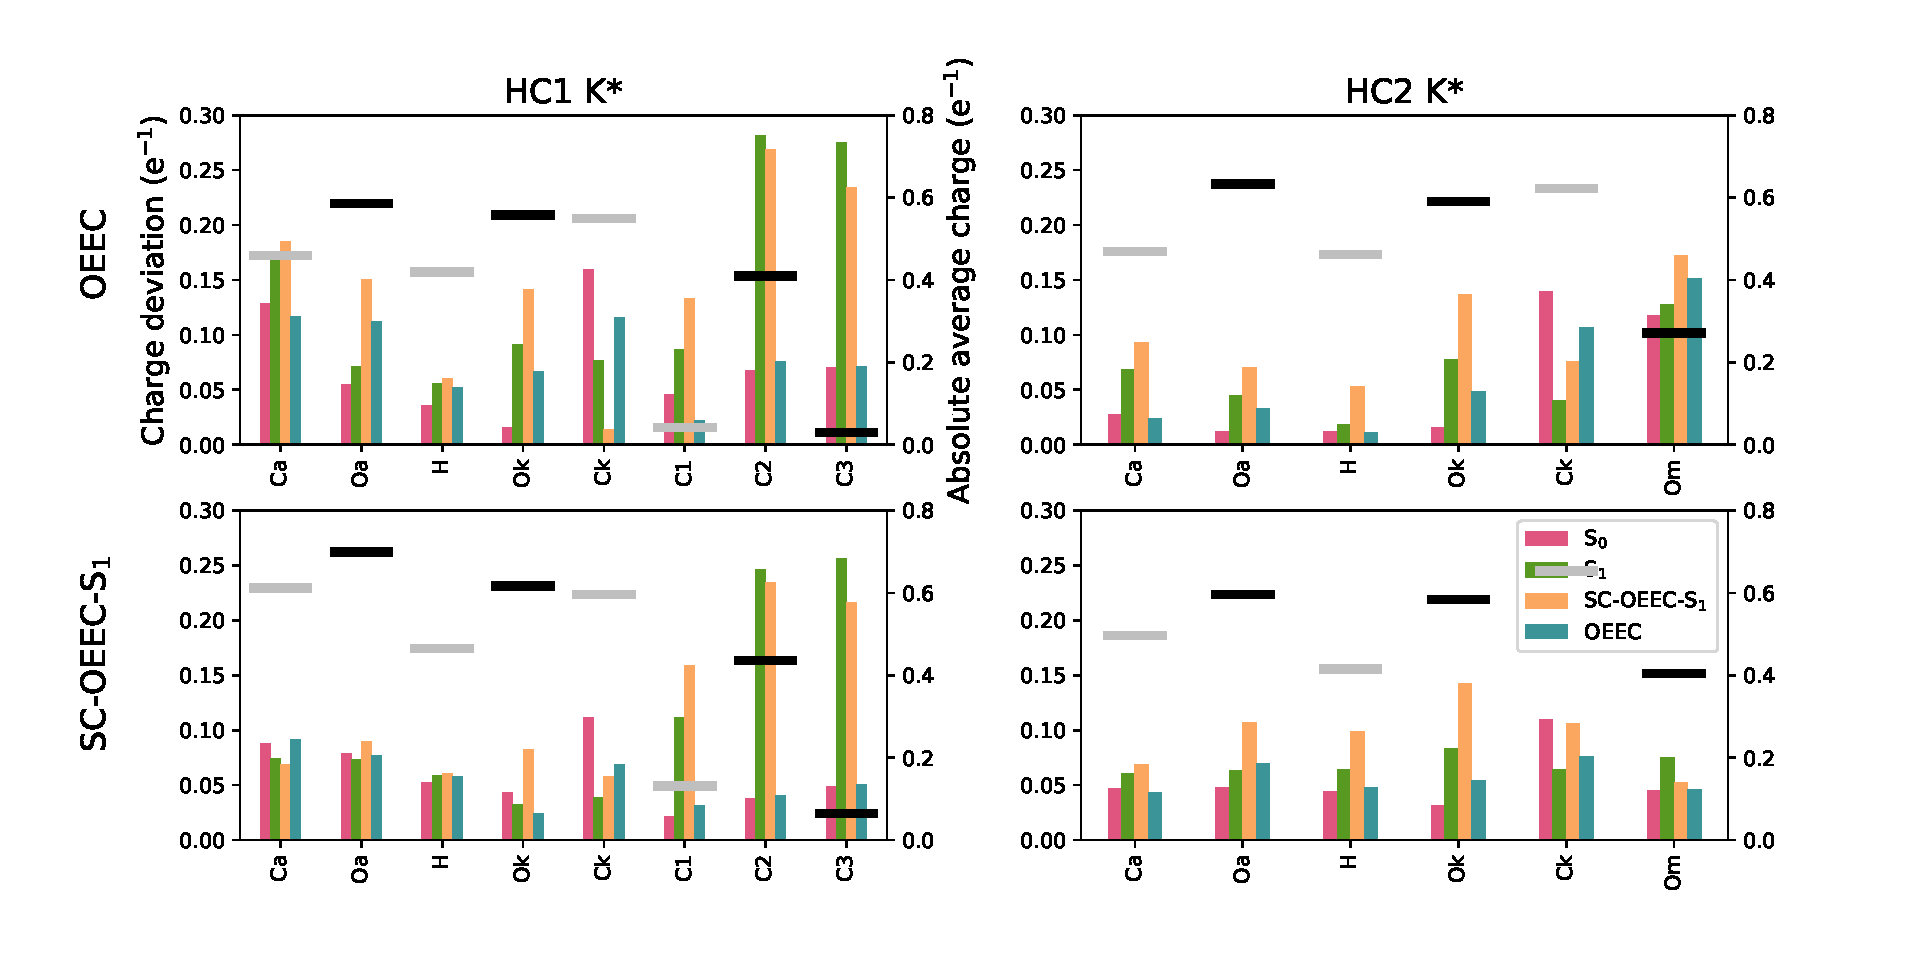
\includegraphics[width=\textwidth]{Appendices/A/just_K.pdf}
\caption{Deviation of charge on notable atoms from the explicitly calculated tetramer with the relaxing molecule in \textbf{K*} geometry. In the top row, the molecule is optimised with \EEC{} and in the bottom with \SCEEC{}-S$_1$. We compare the charge obtained from the monomer population analysis of in vacuum S$_0$, S$_1$ and in EEC and \SCEEC{}-S$_1$. The absolute average charge in the tetramer is indicated by horizontal ticks, positive values are in grey and negative ones in black. The atom labels are the ones found in Figure 1 of the main text.}
\label{fig:chargesK}
\end{figure}


\begin{figure}[H]
\centering
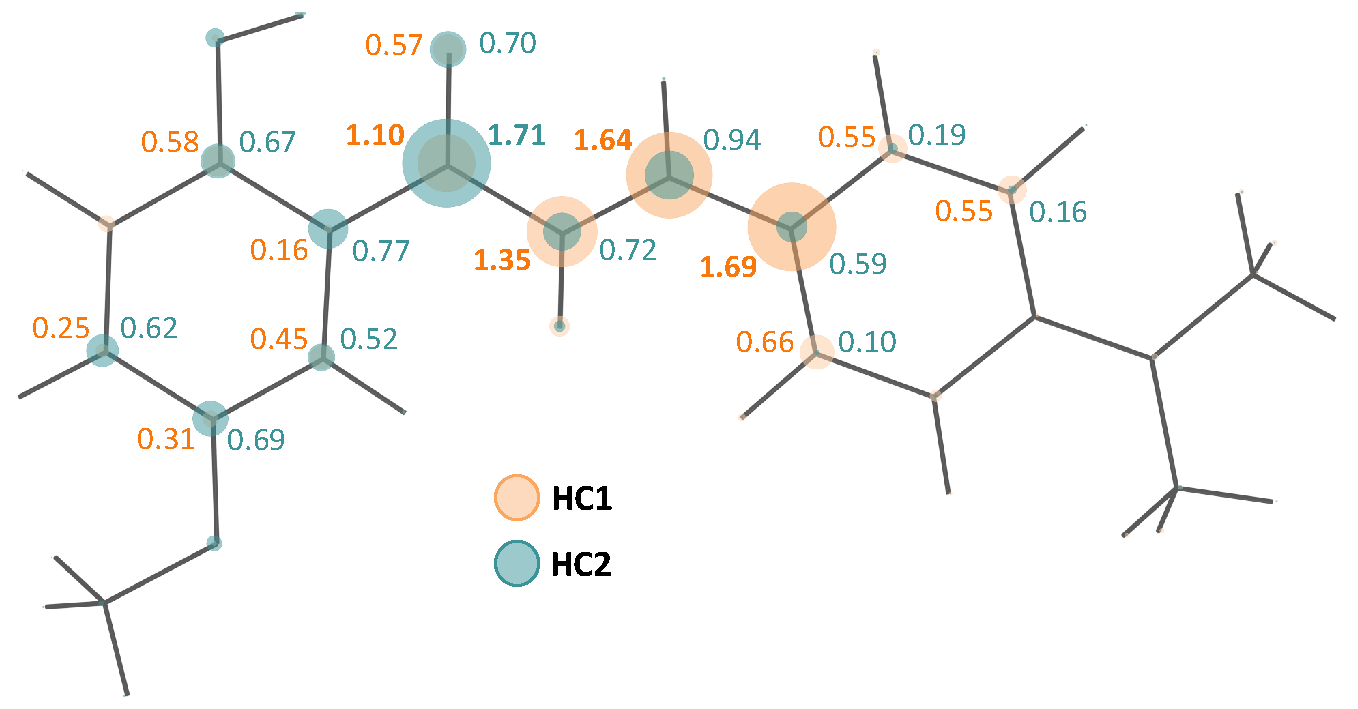
\includegraphics[width=10cm]{Appendices/A/charge_diff.pdf}
\caption{Largest differences in RESP charges between S$_1$ and S$_0$ for HC1 and HC2 in vacuum in units of 10$^{-1}$ e$^{-1}$. We only include atoms where the difference was more than 0.01 e$^{-1}$ in either molecule. The diameter of the circles is proportional to the charge difference.}
\label{fig:char_diff}
\end{figure}
\section{Vertical Excitation for Aggregate}
\label{app:sec:tetramer_vert}

The bright state of \HCC{} has a different identity depending on the charge background. We illustrate this in Figs \ref{fig:hc1abs} and \ref{fig:hc2abs}.

\begin{figure}[H]
%\centering
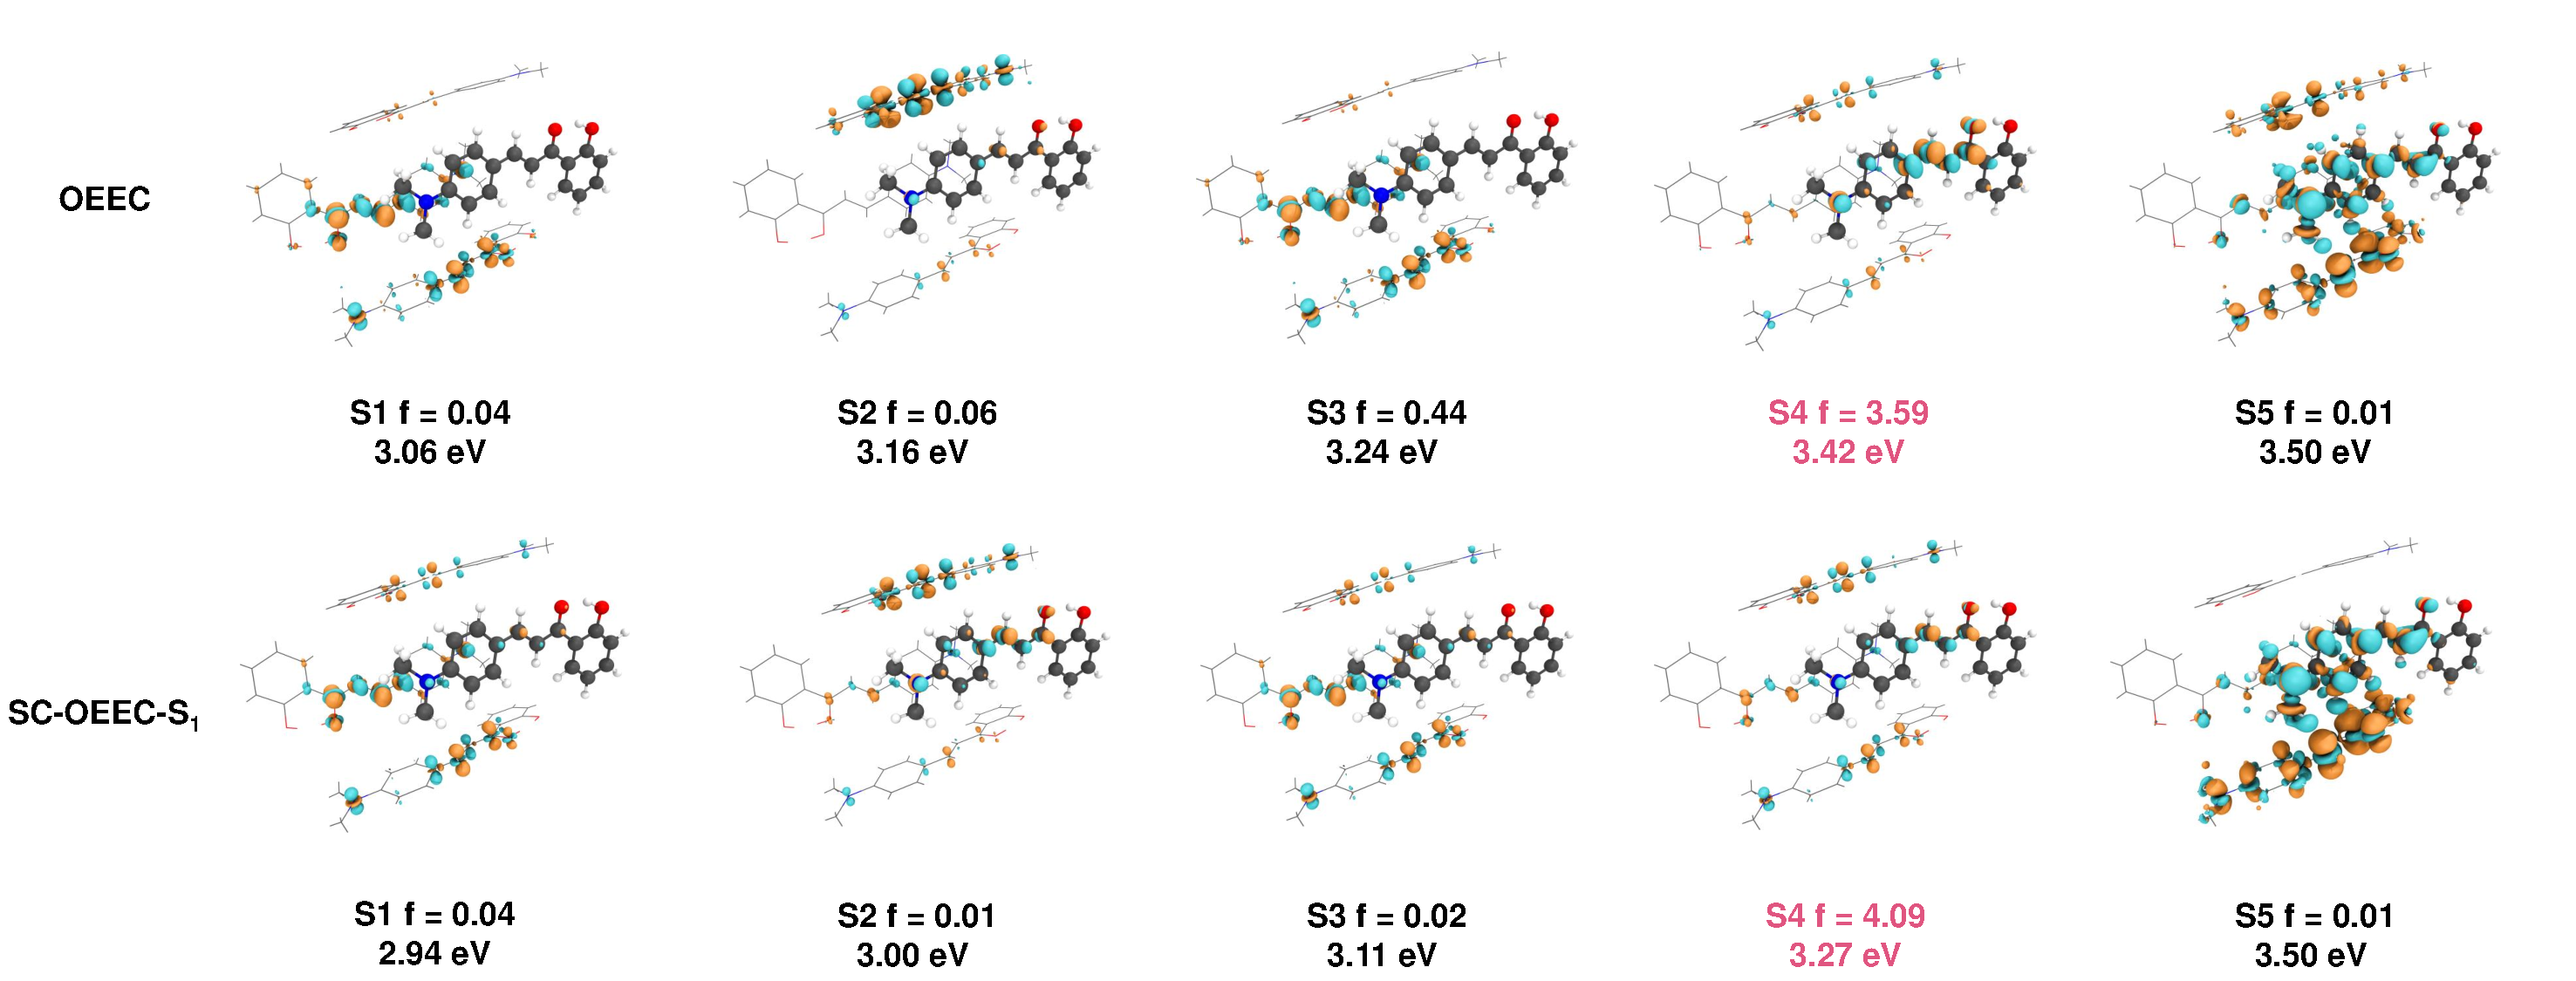
\includegraphics[width=16cm]{Appendices/A/HC1abs_vertical.pdf}
\caption{Density plots for the absorption of HC1 under \EEC{} and \SCEEC{}. The for each excited state $n$, the difference in electronic density S$_n$\textendash{}S$_0$ is plotted where positive values are shown in orange and negative values in blue. The bright state is highlighted in pink.}
\label{fig:hc1abs}
\end{figure}

\begin{figure}[H]
%\centering
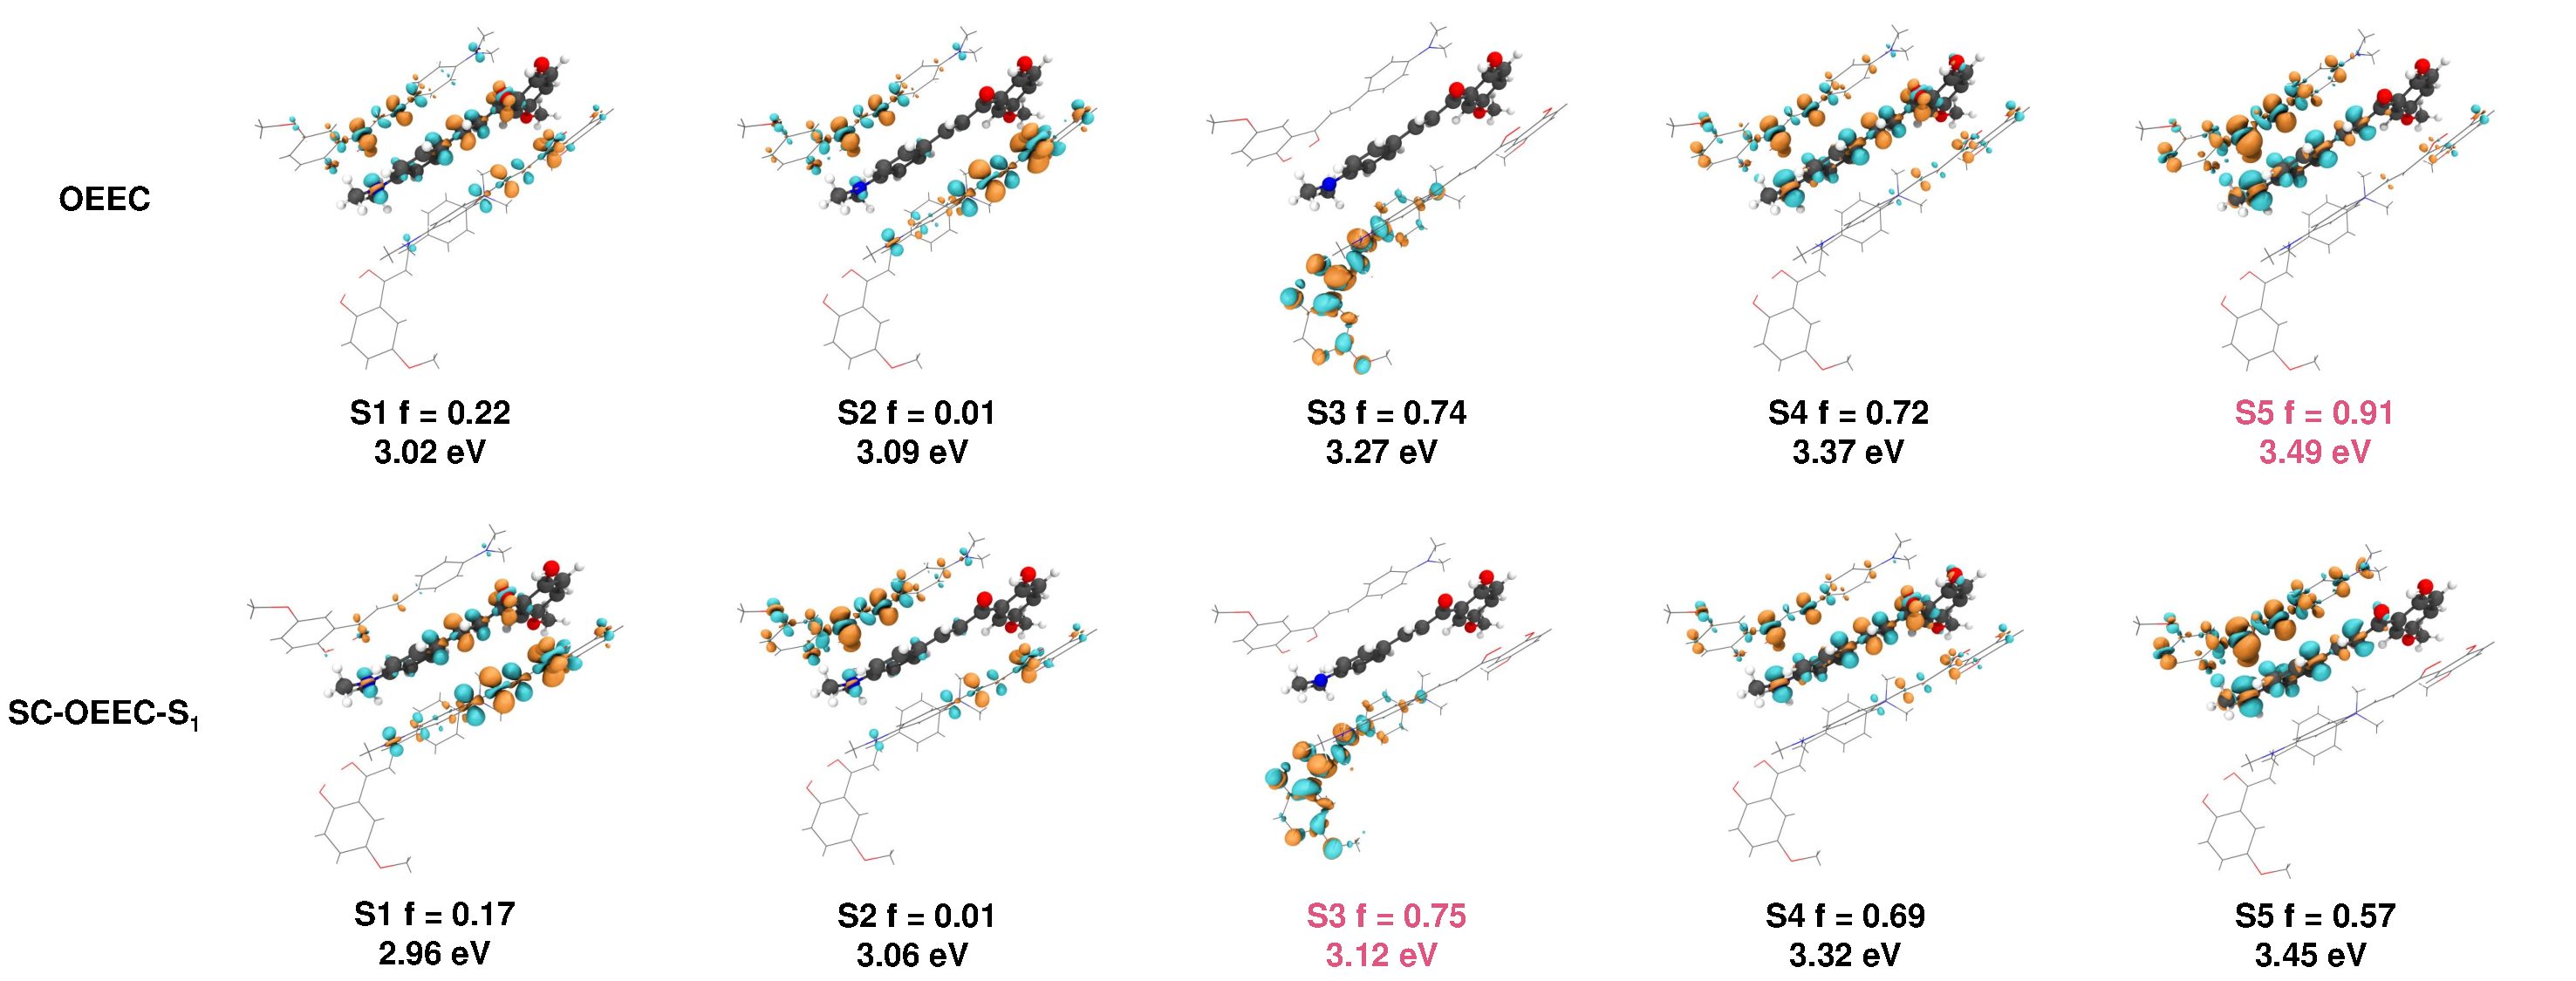
\includegraphics[width=16cm]{Appendices/A/HC2abs_vertical.pdf}
\caption{Density plots for the absorption of HC2 under \EEC{} and \SCEEC{}. For each excited state $n$, the difference in electronic density S$_n$\textendash{}S$_0$ is plotted where positive values are shown in orange and negative values in blue. The bright state is highlighted in pink.}
\label{fig:hc2abs}
\end{figure}

\section{Exciton Coupling in Dimers}
\label{app:sec:troisi_J}


Dimeric exciton couplings were computed using the diabatisation scheme devised by Aragó and Troisi.\cite{Arag2015} In this scheme, a diabatisation excited state property is selected. (1) It is first evaluated for the dimer in S$_1$ and S$_2$, along with the excited state energy. (2) It is also calculated for the constituent monomers of the dimer. (3) Then, a singular-value decomposition is employed to determine the matrix which best transforms the property from the adiabatic to the diabatic basis. (4) Finally, the newly obtained diabatisation matrix is used to transform the adiabatic Hamiltonian into the diabatic one. The latter's off-diagonal elements are the desired J exciton coupling values. 

More details are offered in section \ref{sec:detail_js}. The results for HC1 and HC2 are shown in Table \ref{tab:couplings}. Also shown are the couplings obtained using half of the energy gap between S\textsubscript{1} and S\textsubscript{2} in the dimer.

\begin{table}[H]
\centering
\caption{Exciton couplings (eV) for the different fragments involved in the tetramers computed with the diabatisation scheme. In parenthesis is half the energy splitting between S\textsubscript{1} and S\textsubscript{2}.  The dimers A, B and C are shown in the Figure 6 of the main text} 
\label{tab:couplings}
\begin{tabular}{ccc}
\toprule
\textbf{Dimer} & \textbf{HC1} & \textbf{HC2}\\\midrule
A & 0.012 (0.012) & 0.116 (0.117)\\
B & 0.108 (0.109) & 0.148 (0.148)\\
C & 0.061 (0.063) & 0.001 (0.003)\\\bottomrule
\end{tabular}
%}\par
%\end{adjustwidth}
\end{table}
\section{Results with CC2 and CASPT2}
\label{app:sec:cc2_caspt2}

\begin{table}[H]
\centering
\small
\captionof{table}{Table of absorption and emission energies with RI-CC2 and multireference methods for both model systems after geometry optimisation. The energies are in eV}
\label{tab:em_abs_cas}
%\begin{adjustwidth}{-1.8cm}{}
%\resizebox{\textwidth}{!}{
%\begin{tabular}{@{}c>{\centering\arraybackslash}mcccc@{}}
\begin{tabular}{@{}cp{8cm}cccc@{}}
%\begin{tabular}{@{}cccccc@{}}

\toprule
\multirow{2}{*}{\textbf{Cluster model}}& \multicolumn{1}{c}{\multirow{2}{*}{\textbf{Method}}}& \multicolumn{2}{c}{\HC{}}                 & \multicolumn{2}{c}{\HCC{}}   \\ \cmidrule(lr){3-4} \cmidrule(lr){5-6}
& & \multicolumn{1}{c}{\textbf{FC}}               & \multicolumn{1}{c}{\textbf{K*}}           & \multicolumn{1}{c}{\textbf{FC}}          & \multicolumn{1}{c}{\textbf{K*}}              \\ \midrule
\multirow{4}{*}{\EEC{}}&RI-CC2\slash{}TZVP
& 2.99  & 1.08 & 3.11 & 0.97 \\
&RI-CC2\slash{}TZVP\slash{}\slash{}TD-$\omega$B97X-D\slash{}6-311++G(d,p)
& 3.08 & 1.48 & 3.20 & 1.62 \\
%&CASSCF\slash{}6-31G(d)
%& 4.25 & 1.03  & - & - \\
&CASPT2\slash{}6-31G(d)\slash{}\slash{}CASSCF\slash{}6-31G(d)
& 3.53 & 1.41 & - & - \\
&CASPT2\slash{}6-31G(d)\slash{}\slash{}TD-$\omega$B97X-D\slash{}6-311++G(d,p)
& 3.52 & 1.74 & - & - \\\midrule

\multirow{4}{*}{\SCEEC{} S$_1$} & RI-CC2\slash{}TZVP
& 2.61 & 1.41 & 2.99 & 1.03 \\
&RI-CC2\slash{}TZVP\slash{}\slash{}TD-$\omega$B97X-D\slash{}6-311++G(d,p)
& 2.68 & 2.19 & 3.07 & 1.73 \\
%&CASSCF\slash{}6-31G(d)
%& 3.65 & 1.31 & - & -\\
&CASPT2\slash{}6-31G(d)\slash{}\slash{}CASSCF\slash{}6-31G(d)
& 3.06 & 1.50 & - & -\\
&CASPT2\slash{}6-31G(d)\slash{}\slash{}TD-$\omega$B97X-D\slash{}6-311++G(d,p)
& 3.01 & 2.27 & - & - \\\midrule

\bottomrule
\end{tabular}
%}\par
%\end{adjustwidth}
\end{table}
